\subsection{Hidden Unit as Feature Detectors}
If we consider the \textit{trigonometric} form of the pre-activation function $z = \mathbf{w^Tx} + b
= ||w||\ ||x||cos\theta + b$ where $\theta$ is the angle between $\mathbf{w}$ and $\mathbf{x}$. 
For inputs of similar length, z is largest when $\mathbf{x}$ has the same direction of
$\mathbf{w}$, so each hidden unit is a learned \textbf{template}. The bias estabilish how much strict 
must be the correspondence for the unit to be activated. In the example showed in Fig 
\ref{fig:h_as_feat_det}, the first layer units' become detectors of strokes (es. vertical lines) 
\begin{figure}[H]
    \centering
    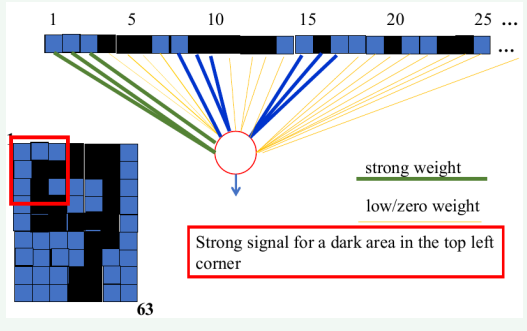
\includegraphics[width=0.7\linewidth]{immagini/h_as_feat_det.png} 
    \caption{An 8x8 digit image flattened into 64 inputs}
    \label{fig:h_as_feat_det}
\end{figure}
\noindent
The limitation is that a unit is tied to fixed pixel position, so the same stroke elsewhere needs another unit.

\subsection{Choosing the hidden unit}
Every hidden unit can be described as accepting a vector of inputs $\mathbf{x}$, computing an affine
transformation $\mathbf{z} = \mathbf{W^T}\mathbf{x} + \mathbf{b}$, and then applying an element-wise
non linear function $g(\mathbf{z})$ (\textit{activation function}). 
So units differ only in the activation function, $g$ needs three rules:
\begin{itemize}
    \item non linearity
    \item non zero slope $g^i(\mathbf{z})$
    \item cheap computation
\end{itemize} 
Which $g$ works best is hard to predict, so it is obtained by trial and error.

\subsection{Step Function}
Easiest example of activation function, the slope is 0 everywhere, so the gradient descent gets no
signal.

\begin{figure}[H]
\centering
\begin{tikzpicture}[scale=0.85]
    % Assi coordinati
    \draw[->, >=stealth, gray, thick] (-4.5,0) -- (4.5,0);
    \draw[->, >=stealth, gray, thick] (0,-1.5) -- (0,2);
    
    % Ticks e etichette sugli assi
    \draw (-4,0.1) -- (-4,-0.1) node[below] {$-4$};
    \draw (4,0.1) -- (4,-0.1) node[below] {$4$};
    \draw (0.1,1) -- (-0.1,1) node[left] {$1$};
    \draw (0.1,-1) -- (-0.1,-1) node[left] {$-1$};
    
    % Titolo del grafico
    \node[above] at (0,2.1) {step};
    
    % Tratti della funzione
    \draw[dashed, thick, orange!70!black] (-4,0) -- (0,0);
    \draw[solid, thick, green!40!black] (0,1) -- (4,1);
    
    % Punti di discontinuità (pallino pieno a destra, vuoto a sinistra)
    \fill[green!40!black] (0,1) circle (2pt);
    \draw[orange!70!black, fill=white, thick] (0,0) circle (2pt);
\end{tikzpicture}
\end{figure}

\subsection{Sigmoid and Hyperbolic Tangent Units}
This two type of units are grouped together because they're functions are closely related: $tanh(z) = 2\sigma(2z) - 1$.
The use of the sigmoid as activation function is discouraged due to the fact that it saturates when 
z is very positive or very negative (Fig \ref{fig:comp_models}). When the sigmoid must be used, the hyperbolic tangent activation 
typically performs bettern than the logistic sigmoid.  
\begin{figure}[H]
\centering
% Grafico Sigmoide
\begin{minipage}{0.48\textwidth}
\centering
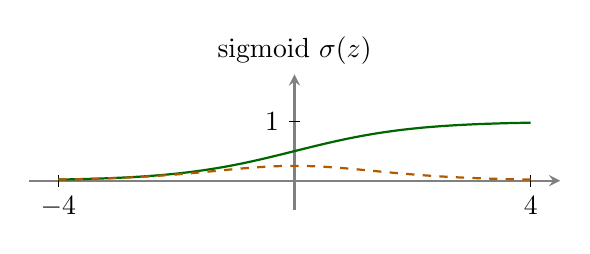
\begin{tikzpicture}[scale=0.75]
    % Assi coordinati
    \draw[->, >=stealth, gray, thick] (-4.5,0) -- (4.5,0);
    \draw[->, >=stealth, gray, thick] (0,-0.5) -- (0,1.8);
    
    % Ticks e etichette
    \draw (-4,0.1) -- (-4,-0.1) node[below] {$-4$};
    \draw (4,0.1) -- (4,-0.1) node[below] {$4$};
    \draw (0.1,1) -- (-0.1,1) node[left] {$1$};
    
    % Titolo
    \node[above] at (0,1.8) {sigmoid $\sigma(z)$};
    
    % Funzione sigmoide: 1 / (1 + e^{-z})
    \draw[green!40!black, thick, domain=-4:4, samples=100] plot (\x, {1/(1 + exp(-\x))});
    
    % Derivata della sigmoide: sigma * (1 - sigma)
    \draw[dashed, orange!70!black, thick, domain=-4:4, samples=100] plot (\x, {(1/(1 + exp(-\x))) * (1 - (1/(1 + exp(-\x))))});
\end{tikzpicture}
\end{minipage}
\hfill
% Grafico Tanh
\begin{minipage}{0.48\textwidth}
\centering
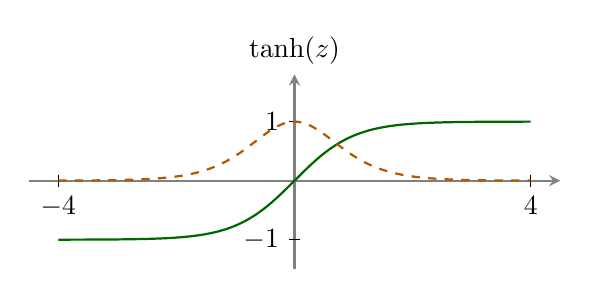
\begin{tikzpicture}[scale=0.75]
    % Assi coordinati
    \draw[->, >=stealth, gray, thick] (-4.5,0) -- (4.5,0);
    \draw[->, >=stealth, gray, thick] (0,-1.5) -- (0,1.8);
    
    % Ticks e etichette
    \draw (-4,0.1) -- (-4,-0.1) node[below] {$-4$};
    \draw (4,0.1) -- (4,-0.1) node[below] {$4$};
    \draw (0.1,1) -- (-0.1,1) node[left] {$1$};
    \draw (0.1,-1) -- (-0.1,-1) node[left] {$-1$};
    
    % Titolo
    \node[above] at (0,1.8) {$\tanh(z)$};
    
    % Funzione tanh(z)
    \draw[green!40!black, thick, domain=-4:4, samples=100] plot (\x, {tanh(\x)});
    
    % Derivata di tanh: 1 - tanh^2(z)
    \draw[dashed, orange!70!black, thick, domain=-4:4, samples=100] plot (\x, {1 - (tanh(\x))^2});
\end{tikzpicture}
\end{minipage}

\vspace{0.3cm}
\centering
\small
\textcolor{green!40!black}{\rule{10pt}{2pt}} \textbf{function $g(z)$} \quad 
\tikz[baseline=-.5mm]{\draw[dashed, orange!70!black, thick] (0,0) -- (10pt,0);} \textbf{slope $g'(z)$} \quad $z \in [-4, 4]$
\caption{Sigmoid and hyperbolic tangent activation functions and their derivatives.}
\label{fig:comp_models}
\end{figure}

\subsection{Rectified Linear Units And Their Generalizations}
Those units use the activation function $g(z) = max(0, z)$. Easy to optimize because they
are so similar to linear units with the only difference that ReLU outputs zero across half
its domain. When active, the unit passes the error signal back \textbf{unchanged} (slope 1), 
no saturation on the positive side. 
\newline
ReLU isn't differentiable\footnote{a function is differentiable if can be locally 
approximated by a linear function} at 0, so the software return 1 or 0, in any case 
most of the time when we work with float types it's rare to have a perfect 0 value. 
\newline
When initializing the parameters, it can be a good practice to set all elements of 
$\mathbf{b}$ to a small positive value (i.e. 0.1) in order to avoid the dead units. 
Infact if z < 0 for every training example, the unit always outputs 0, its slope 
is always 0, and its weights never change again.
There are some \textbf{generalization} that are based on using a nonzero slope $\alpha_i$
when $z_i$ < 0: 
\begin{equation}
    h_i = g(z, \alpha)_i\ = max(0, z_i) + \alpha_imin(0, z_i)   
\end{equation}
and they are:
\begin{itemize}
    \item Absolute value: $\alpha = -1$ and so $g(z) = |z|$, used for object recognition from images
    \item Leaky ReLU: $\alpha = 0,01$
    \item Parametric ReLU $\alpha$ is learned, the data choose the leak.
\end{itemize}
One further generalization is the \textbf{Maxout units}, instead of applying an element-wise
function $g(z)$, maxout units divide $\mathbf{z}$ into groups of $k$ values. A maxout unit
can learn a piecewise linear, convex function with up to k pieces. It of course has a k
times more weights per unit.
\begin{equation}
    h = \max_{j=1,\dots,k} \left( \boldsymbol{w}_j^\top \boldsymbol{x} + b_j \right)
\end{equation}

\subsubsection{Activations in Modern Networks}
Modern networks use a variation of the ReLU that try to minimize the number of dead units,
in Fig \ref{fig:modern_activations} there is a summarize of the 3 variations.
\newline
The difference between ReLU and GELU is the fact that GELU multiplies z by a soft gate
while ReLU uses a hard gate. Thanks to this GELU gains fewer dead units.
\newline
Infact \textbf{ReLU} is defined as:
\begin{equation}
\text{ReLU}(z) = z \cdot \mathbb{1}[z > 0]
\end{equation}
and \textbf{GELU} is defined as:
\begin{equation}
\text{GELU}(z) = z \Phi(z), \quad \Phi(z) = P(Z \leq z), \quad Z \sim \mathcal{N}(0, 1)
\end{equation}
\textbf{SwiGLU} (Swish-Gated LU) the idea is similar as GELU, with $\sigma$ in place 
of $\Phi$: $\text{SiLU}(z) = z \sigma(z)$. In GELU and SiLU the gate depends on $z$ 
\textbf{itself}. In SwiGLU a \textbf{second linear map} of the input computes it:
\begin{equation}
\boldsymbol{h} = \underbrace{\left( \boldsymbol{W}_a^\top \boldsymbol{x} \right)}_{\text{content }\boldsymbol{a}} \odot \underbrace{\text{SiLU}\left( \boldsymbol{W}_b^\top \boldsymbol{x} \right)}_{\text{gate }\boldsymbol{s}}, \qquad \hat{\boldsymbol{y}} = \boldsymbol{W}_2^\top \boldsymbol{h}
\end{equation}
\begin{figure}[H]
    \centering
    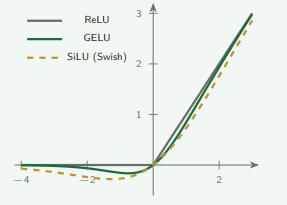
\includegraphics[width=0.7\linewidth]{immagini/relu.png} 
    \caption{Comparison between activation functions}
    \label{fig:modern_activations}
\end{figure}

In conclusion, when using ReLU or a variant, the rule is to pick random and small 
weights and small biases (i. e. 0,01). It is important not to start with weights equal
to 0 because other wise the gradient would \textbf{vanish}. It is important not to 
pick a too large weights neither because otherwise the gradient would \textbf{explodes}.
THe idea is to choose them from a set $Var(w)$ ruled by a variance value, there are two main 
formulations:
\begin{itemize}
    \item Glorot: $\frac{2}{n_{in} + n_{out}}$
    \item He: $\frac{2}{n_{in}}$
\end{itemize}  
where n is the number of inputs per unit.